% !TEX root = /home/jd18380/Documents/compass_yr1/Stat_methods/Portfolio/Section_2/main.tex
\documentclass[a4paper]{article}

%% Language and font encodings
\usepackage[english]{babel}
\usepackage[utf8x]{inputenc}

\usepackage{booktabs}
\usepackage{tabu}
\usepackage[T1]{fontenc}
\usepackage{subfig}

%% Sets page size and margins
\usepackage[a4paper,top=2cm,bottom=3cm,left=3cm,right=3cm,marginparwidth=2.75cm]{geometry}
%% Useful packages
\usepackage{amsmath}
\usepackage{amsfonts}
\usepackage{amssymb}
\usepackage{bm}
\usepackage{xcolor}
\DeclareMathOperator*{\argmax}{arg\!\max}
\DeclareMathOperator*{\argmin}{arg\!\min}
\usepackage[toc,page]{appendix}
\usepackage{graphicx}
%\usepackage{apacite}
\usepackage[colorinlistoftodos]{todonotes}
\usepackage[colorlinks=true, allcolors=blue]{hyperref}
\usepackage{cleveref}

\newtheorem{theorem}{Theorem}[section]
\newtheorem{corollary}{Corollary}[theorem]
\newtheorem{lemma}[theorem]{Lemma}
\newtheorem{definition}{Definition}[section]
\newtheorem{question}{Question}[subsection]

\newcommand{\yi}{y_{i}}
\newcommand{\gxi}{g_{\bm{x}_{i}}}
\newcommand{\gx}{g_{\bm{x}}}
\newcommand{\ei}{\epsilon_{i}}
\newcommand{\E}{\mathbb{E}}
\newcommand{\wls}{\bm{w}_{LS}}
\newcommand{\wlsr}{\bm{w}_{LS-R}}
\newcommand{\wmap}{\bm{w}_{MAP}}
\newcommand{\xui}{\bm{x}_{i}}
\newcommand{\prls}{f(\xui ; \wls)}
\newcommand{\prlsv}{f(\bm{x} ; \wls)}
\newcommand{\V}{\text{Var}}
\newcommand{\y}{\bm{y}}
\newcommand{\x}{\bm{x}}
\newcommand{\w}{\bm{w}}
\newcommand{\F}{\bm{\phi}}
\newcommand{\I}{\bm{I}}
\newcommand{\X}{\bm{X}}
\newcommand{\K}{\bm{K}}
\newcommand{\yh}{\hat{y}}
\newcommand{\dpost}{\Delta \textit{posterior}}
\newcommand{\dprior}{\Delta \textit{prior}}


\title{Statistical Methods: Portfolio 2}
\author{By Henry Bourne}
\date{}

\begin{document}
\maketitle


% \begin{abstract}
%     In this document we will summarize content from the first 4 lectures from the Statistical methods course (at Compass, University of Bristol). These lectures cover content on using statistical methods for decision-making.
% \end{abstract}

\section*{Question 0}
E

\section*{Question 1}

\subsection*{1.1}
The answer is c or d as this line goes roughly through the class means and when the data points are projected onto the embedding vector (for either of the directions) it appears as though the between-class scatterness will be maximized and the within-class scatterness minimized as points from the negative/positive class will be close together and the class means in the embedding will be fairly centrally located (within their classes). For comparison we can argue that the opposite would be true for directions a and b, where points from both classes will not be separated (class-wise) in the embedding and the furthest points from a given class to its class mean will be larger than we had with embedding vectors in directions c or d. 

\subsection*{1.2}
We can construct a likelihood function over the entire dataset:
\begin{equation}
    L(\bm{\mu},\bm{\Sigma}) := \prod_{i=1}^{n} p(\xui | \bm{\mu}, \bm{\Sigma}) = \prod_{i=1}^{n} N_{\xui}(\bm{\mu},\bm{\Sigma})
\end{equation}
ie. all the points are iid. normally distributed (have same mean and covariance matrix) where $\bm{\Sigma}_{ML}$ maximizes the above likelihood.

Let's take the decomposition to be the eigen-decomposition of $\bm{\Sigma}_{ML}$, then $\bm{\mu}_{1}$ is an eigenvector of $\bm{\Sigma}_{ML}$ with corresponding eigenvalue $D_{1}$. Note that $D_{1} > D_{2}$ which means the eigenvector $\bm{u}_{1}$ corresponds to the direction of the largest variance in the data, hence must correspond to direction a or b. 

\section*{Question 3}
Recall the soft margin SVM:
\begin{align}
    \text{Minimize} \: \: || \w '||^{2} + \sum_{i \in D} \epsilon_{i} \\
    \text{Subject to} \: \: \forall i, y_{i} \cdot f(\xui ; \w) + \epsilon_{i} \geq 1, \epsilon_{i} \geq 0
\end{align}
We can modify the objective function such that it penalizes False Negatives (FN) by making FNs 1000 times more costly by rewriting the objective function as:
\begin{equation}
    \text{Minimize} \: \: || \w ' ||^{2} + \sum_{i \in D} (1000 \cdot I(y_{i}=1) + (1-I(y_{i}=1))  )\cdot \epsilon_{i}
\end{equation}
where $I(y_{i}=1)$ is the indicator function that is one when $y_{i}=1$ (ie. when wrongly classifying would lead to a FN) it multiplies the cost times 1000. So, during optimization we will have attributed a 1000x cost to giving a FN, meanwhile the cost of a FP stays as is (a 1000th of the cost).

\section*{Question 4}
\subsection*{4.1}
B
\subsection*{4.2}
The factorization of $p(y,x^{(1)},x^{(2)},x^{(3)},x^{(4)})$ according the to graph is:
\begin{equation}
    p(y) \cdot p(x^{(1)}|y) \cdot p(x^{(2)}|y,x^{(1)}) \cdot p(x^{(3)}|x^{(2)}) \cdot p(x^{(4)}|x^{(1)}) 
\end{equation}
The conditional independencies encoded by this graph are:
\begin{align}
    x^{(2)} \bot x^{(4)} | y,x^{(1)} \\
    x^{(3)} \bot y,x^{(1)},x^{(4)} | x^{(2)} \\
    x^{(4)} \bot y, x^{(2)}, x^{(3)} | x^{(1)}
\end{align}
And no we should just use $x^{(1)}$ and $x^{(2)}$ as given these two features we have from our conditional independencies that $x^{(3)}$ and $x^{(4)}$ are independent of y, we also have that our prediction function:
\begin{align}
    p(y|x^{(1)},x^{(2)},x^{(3)},x^{(4)}) &{} = \frac{p(y) \cdot p(x^{(1)}|y) \cdot p(x^{(2)}|y,x^{(1)}) \cdot p(x^{(3)}|x^{(2)}) \cdot p(x^{(4)}|x^{(1)})}{p(x^{(1)},x^{(2)},x^{(3)},x^{(4)})} \\
    &\propto p(y) \cdot p(x^{(1)}|y) \cdot p(x^{(2)}|y,x^{(1)})
\end{align}
Therefore to formulate a prediction for y we only need $x^{(1)}$ and $x^{(2)}$.
\section{Stein Variational Gradient Descent: A General Purpose Bayesian Inference Algorithm \cite{liu2016stein}}
This paper proposes a general purpose variational inference algorithm that in empirical studies performs competitively with the existing state-of-the-art methods at the time (2019). The derivation of the method is based on a new theoretical result that connects the derivative of the KL divergence under smooth transforms with Steins identity aswell as a  kernelized Stein discrepancy. 

We will begin by first asking what is variational inference? \textbf{Variational inference} concerns methods that approximately infer a probability distribution. In particular we seek to infer a distribution that is close to the true posterior distribution of the model but is tractable and easy to work with. This is typically done by defining a family of distributions and then finding the member of that family that is ``closest'' to the true posterior in some sense. 

More mathematically: we want to find a distribution $q$ that is approximately $p$, ie. $q \approx p$, where p is our target distribution. Let $x$ be a continuous random variable or parameter of interest and D be our dataset consisting of iid observations. We would like to find the posterior of x, ie. $p(x|D)$. One potential way to find the posterior would be using sampling methods such as Markov Chain Monte Carlo (MCMC) methods. With these methods we generate samples from the posterior distribution, ie. we generate $x_{i} \sim p(x|D)$, and then use these samples to approximate the posterior. However, these methods can be very computationally expensive, especially for high-dimensional models amongst other disadvantages.

Another way of finding the posterior is to find some $q$ that minimizes the Kullback-Leibler divergence: $\min_{q \in F} \text{KL}(q,p)$, where F is some set of distributions that we restrict ourselves to. This approach is defined by variational inference.

However, does there exist a more flexible approach? one where we are not restricted to F (is non-parametric)? let $X \sim Q$ where $Q$ has density $q(x)$ and let $X'=X+ \epsilon V(X)$, where $V \in \mathbb{R}^{d} \sim Q'$ has density $q'(x)$. What we are doing here is we are saying $x$ comes from some proposal distribution Q, we are then ``moving'' our samples (or particles) by some magnitude $\epsilon$ in direction given to us by $V$ in the hope that the distribution of our now moved samples is closer to that of the true distribution. To ``move our samples'' in the optimal direction we would like to choose $V$ such that $\text{KL}(q',p) < \text{KL}(q,p)$ and the optimal V will decrease the KL divergence by the maximum amount (ie. minimize it). What we are doing in this process is carrying out gradient descent.

So, we would like to find $\min_{V, ||V||=1} \wrte \KL(q',p)|_{\epsilon=0}$. First, note that by the law of the unconscious statistician,
\begin{equation}
    \KL(q',p) = \mathbb{E}_{x'} \left(\log \left(\frac{q'(x')}{p(x')} \right) \right) = \mathbb{E}_{x} \left(\log \left(\frac{q(x+ \epsilon V(x))}{p(x+\epsilon V(x))} \right) \right)
\end{equation}
We then have that,
\begin{equation}\label{equation:eq1}
    \mathbb{E}_{x} \left( \log \left(\frac{q(x+ \epsilon V(x))}{p(x+\epsilon V(x))} \right) \right)
    = E_{x} \left( \frac{\log (q(x+ \epsilon V))}{\log(p(x+ \epsilon V))} \right)
    + E_{x}(\log q'(x+ \epsilon V(x)) ) - E_{x}(\log q(x+ \epsilon V(x)) )
\end{equation}
We will now state a lemma which will get rid of the added cost (the last two terms):
\begin{lemma}\label{lemma:one}
    $\wrte \mathbb{E}_{x}(\log \frac{q'(x + \epsilon V(x))}{q(x+ \epsilon V(x))})|_{\epsilon=0} = 0$
\end{lemma}
The proof of this lemma is in \ref{Proofs:one}. We can then split the first term on the RHS in \ref{equation:eq1} and take the derivative to get:
\begin{equation}
    \wrte[ \mathbb{E}_{x}[\log q(x+ \epsilon V(x))] - \mathbb{E}_{x}[\log p(x + \epsilon V(x))]]
\end{equation}
First lets look at the first term above:
\begin{align}
    \wrte \mathbb{E}_{x}[\log q(x+ \epsilon V(x))]|_{\epsilon=0} &{}
    = \mathbb{E}_{x}[\wrte \log q(x + \epsilon V(x))]|_{\epsilon=0} \\
    &= \mathbb{E}_{x} \left[\frac{\wrte q(x + \epsilon V(x))}{q(x+ \epsilon V(x))} \right] \bigg\rvert_{\epsilon=0} \\
    &= \mathbb{E}_{x} \left[\frac{\langle \wrtx q(x+\epsilon V(x)), V(x) \rangle }{q(x+ \epsilon V(x))} \right] \bigg\rvert_{\epsilon=0} 
    \text{\footnotemark}\\
    &= \mathbb{E}_{x} \left[\frac{\langle \wrtx q(x), V(x) \rangle}{q(x)} \right] \\
    &= - \mathbb{E} \left[\sum_{i} \frac{\partial}{\partial x_{i}} V_{i}(x) \right]
\end{align}
\footnotetext{We get this step by using the directional derivative, that is we have by the chain rule that $\frac{\partial}{\partial \epsilon} q(x+ \epsilon V(x)) = \frac{\partial q}{\partial x} \frac{\partial x}{ \partial \epsilon} (x+ \epsilon V(x)) = V(x) \frac{\partial q}{\partial x} (x+ \epsilon V(x))$} 
For the second term we have:
\begin{align}
    - \wrte \mathbb{E}_{x}[\log p(x + \epsilon V(x))] 
    &{}= - \mathbb{E}_{x}\left[\frac{\langle \wrtx p(x + \epsilon V(x)), V(x) \rangle}{p(x+ \epsilon V(x))} \right] \bigg\rvert_{\epsilon=0} \\
    &= - \mathbb{E}_{x} \left[\frac{\langle \wrtx p(x), V(x) \rangle}{p(x)} \right] \\
    &= - \mathbb{E}_{x} \left[\sum_{i} \frac{\partial}{\partial x_{i}} \log p(x) V_{i}(x) \right]
\end{align}
Where $V(x) \in \mathbb{R}^{d}$ with $V_{i}(x) = \langle V, \phi_{i}(x) \rangle$ with $\phi_{i} \in \mathbb{R}^{b}$. Where our $\phi_{i}'s$ are the feature transforms induced by a kernel we choose, this is where the Reproducing Kernel Hilbert Space (RKHS) comes in (which is mentioned many times in the paper) as its induced by the kernel. Therefore,
\begin{align}
    \wrte \KL(q',p) &{}= - \mathbb{E}_{x}[\langle V, \sum_{i} \frac{\partial}{\partial x_{i}} \log p(x) \phi_{i}(x) \rangle ] - \mathbb{E}_{x}[\langle V, \sum_{i} \frac{\partial}{\partial x_{i}} \phi_{i}(x) \rangle ] \\ 
    &= \langle V, -\mathbb{E}_{x}[\sum_{i} \log p(x) \phi_{i}(x) + \sum_{i} \frac{\partial}{\partial x_{i}} \phi_{i}(x) ] \rangle
\end{align}
We want to minimize $\wrte \KL(q',p)$ subject to $||V||=1$. So we take our optimal value for v, $V^{*}$, to be:
\begin{equation}
    V* = \frac{\mathbb{E}_{x}[ \sum_{i} \log p(x) \phi_{i}(x) + \sum_{i} \frac{\partial}{\partial x_{i}} \phi_{i}(x) ]}{ || \mathbb{E}_{x}[\sum_{i} \log p(x) \phi_{i}(x) + \sum_{i} \frac{\partial}{\partial x_{i}} \phi_{i}(x)] ||}
\end{equation}
Where we obtain the expectation using MCMC (note its cheaper here than it would be using it directly on the posterior). Now we can construct an algorithm:
\begin{enumerate}
    \item $\{x_{0}^{n}\}_{n=1}^{N} \sim Q_{0} $
    \item For $i = 1,...,100$
    \begin{enumerate}
        \item $x_{i+1}^{n} = x_{i}^{n} + \epsilon \cdot V^{*}(x_{i}^{n})$
    \end{enumerate}
\end{enumerate}
Where we find $V^{*}$ as we defined above. Using this we can then perform variational inference. 
\section{Bayesian Network (Directed Graph)}\label{section:Bayesian-Network}
So far we have been working with undirected graphs to represent conditional independencies. However, what if we want to represent causal relationships for example? then what might serve as a better model would be a directed graphical model, we will be using a:
\begin{definition}
    \textbf{Directed Acyclic Graph (DAG):} \\
    A graph, $G = (V,E)$, where $E$ is a directed edge set and $G$ is an acyclic graph, ie. it has no directed cycles. 
\end{definition} 
We can represent the factorization of a probability distribution using a DAG. We say a probability distribution $p(X)$ factorizes over a DAG $G$ if $p(X) = \prod_{v \in V} p(X_{v} | X_{ \text{parent}(X_{v}) })$. And we can construct the DAG using a similar methodology to constructing undirected graphical models.

We can also represent conditional independencies using a DAG. Given a DAG $G$, $X_{v}$ is independent of $X_{\text{non-desc}(X_{v})}$ given $X_{\text{parent}(X_{v})}, \forall v$. This is analogous to the markov net as $X_{v}$ and all non-descendants of $X_{v}$ are "made independent" by the parents of $X_{v}$. Also note that knowing $X_{\text{parent}(X_{v})}, X_{\text{non-desc}(X_{v})}$ tell us nothing new about $X_{v}$. Just as in \cref{section:sectionone} we can show that the graph given by the dependencies and the graph given by the factorization are equivalent.

We can then define a:
\begin{definition}
    \textbf{Bayesian Network:} \\
    A DAG $G$ constructed using the factorization of a probability distribution, $p(\x)$.
\end{definition}
Lets consider again the simple graph described in \cref{subsubsection:Logistic-Regression} except we have a directed edge (instead of undirected) going from $Y$ to each $X^{(i)}$. We can write down the conditional probability from this graph:
\begin{equation}
    P(Y|X) = \frac{\prod_{i} P(X^{(i)} | Y) P(Y)}{P(X)}
\end{equation}
Note that this is how Naive Bayes is derived.

\subsection{Bayesian Network for Classification vs. Logistic Regression}
Consider the setup with the simple graph we just introduced, we note that it has the same structure as the graph that lead to a logistic regression, except the edges were directed. What are the similarities and differences between naive Bayes and logistic regression? 

First lets consider the factorization, for both we have pairwise factors between Y and the $X^{(i)}$. However, in Naive Bayes the factors are conditional probabilities as opposed to cliques in logistic regression. Next, we have that for the probabilistic model they both use $p(Y|X)$ to make a prediction, however, Naive Bayes does not give you $p(Y|X)$ it only give you it up to a constant. Next, for the training/fitting of the classifier in the logistic regression case we estimate $p(Y|X)$ as opposed to $P(X|Y)$ in the case of naive bayes. Finally, for both we use the prediction rule: $\hat{y} := \argmax_{y} p(Y|X)$.
\newpage
\begin{appendices}


% \section{Proofs}

% \subsection{---} \label{Proofs:}



%\newpage
\section{Homeworks}
\subsection{For Section 1}

\begin{question}\label{question:graph-equivelance}
    \textbf{Show equivalence between the factorization and conditional independence over G in the Scores of units example:} \\
    First we will create G using the following factorization:
    \begin{equation}
        p(\text{Maths}, \text{SM}1, \text{Python}, \text{ML}) \propto g_{1}(\text{Maths}, \text{SM}1) \cdot g_{2}(\text{Python}, \text{ML}, \text{SM}1)
    \end{equation}
    The graph corresponding to this factorization is:
    \begin{figure}[h]
    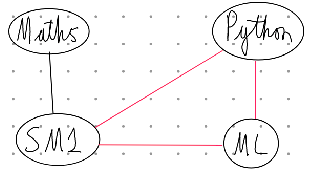
\includegraphics[width=\textwidth/2]{images/factor_graph.png}
    \centering
    \end{figure}
    Where in black is the edges corresponding to the clique given by the first factor and in red the edges corresponding to the clique given by the second factor. The conditional independencies encoded by this graph are:
    \begin{enumerate}
        \item Maths $\bot$ Python $|$ SM1
        \item Maths $\bot$ Python $|$ SM1, ML 
        \item Maths $\bot$ ML $|$ SM1
        \item Maths $\bot$ ML $|$ SM1 , Python
        \item Maths $\bot$ ML, Python $|$ SM1
    \end{enumerate}
    Which are all the conditional independencies of $p(\text{Maths}, \text{SM}1, \text{Python}, \text{ML})$. 

    Now we will create G using all the conditional independencies, which are:
    \begin{enumerate}
        \item Maths $\bot$ Python $|$ SM1
        \item Maths $\bot$ Python $|$ SM1, ML 
        \item Maths $\bot$ ML $|$ SM1
        \item Maths $\bot$ ML $|$ SM1 , Python
        \item Maths $\bot$ ML, Python $|$ SM1
    \end{enumerate}
    The graph we get is the same as before, and reading the graph its clear that it encodes the factorization of $p(\text{Maths}, \text{SM}1, \text{Python}, \text{ML})$. Hence, shown.
\end{question}

\subsection{For Section 2}
\begin{question}
    \textbf{Suppose graph G encodes all conditional independencies in your Gaussian distribution $p(\x)$. Let's say G contains 3 edges and 5 nodes. How many non-zero elements are there in inverse covariance matrix of p?:} \\
    There are 25 entries in $\bm{\Theta}$ and in the adjacency matrix of G (also with 25 entries) there are 6 non-zero (ie. equal to 1) entries hence only 6 entries in $\bm{\Theta}$ that are non-zero (from \cref{equation:adjacency-Theta}). 
\end{question}

\begin{question}\label{question:logistic-regression}
    \textbf{In \cref{subsubsection:Logistic-Regression} we constructed a logistic regression from our simple Markov network model where $\hat{\bm{\beta}}, \hat{\beta_{0}} = \argmax_{\bm{\beta}, \beta_{0}} \sum_{i=1}^{n} \log(p(y_{i}|\xui;\bm{\beta},\beta_{0}))$ show that this is the same logistic regression we talked about in portfolio 3:} \\
    Note that we can write:
    \begin{equation}
        p(y=-1| \x) = 1 / (1+ \frac{p(\x|y=+1)p(y=+1)}{p(\x|y=-1) p(y=-1)})
    \end{equation}
    And for $p(y=-1|\x)$ the same is true but with the inverse of the ratio of the densities. We can rewrite this more generally as:
    \begin{equation}
        p(y | \x; \bm{\beta}, \beta_{0}) = \sigma(f(\x;\bm{\beta}, \beta_{0}) \cdot y)
    \end{equation}
    where $f(\x;\bm{\beta}, \beta_{0}) = log( [p(\x|y=+1)p(y=+1)] / [p(\x|y=-1) p(y=-1)] )$. Hence we can rewrite our MLE as the logistic regression:
    \begin{equation}
        \hat{\bm{\beta}}, \hat{\beta_{0}} = \argmax_{\bm{\beta}, \beta_{0}} \sum_{i=1}^{n} \log (\sigma(f(\xui;\bm{\beta}, \beta_{0}) \cdot y_{i}))
    \end{equation}
    Which is the same logistic regression we had in portfolio 3.
\end{question}


\subsection{For Section 3}
\begin{question}
    \textbf{Given the simple Bayesian Network model described in \cref{section:Bayesian-Network}, however, now with one additional node $X'$ which has one inbound directed edge from $X^{(1)}$. Given this Bayesian Network for a classification task, should you include feature $X'$ for classification? and why?} \\
    To be able to solve the classification problem we would like to find $p(Y|X)$ which for this Bayesian Network is equal to:
    \begin{equation}
        P(Y|X) = \frac{\prod_{i} P(X^{(i)} | Y) P(Y)P(X' | X^{(1)}) }{P(X)}
    \end{equation}
    Hence, we should include feature $X'$ for classification as our factorization and therefore prediction depends on it. 
\end{question}


\end{appendices}

% \small
% \bibliographystyle{plain}
% \bibliography{refs}

\end{document}